
\section{Data}

The \href{https://en.wikipedia.org/wiki/MNIST_database}{\texttt{MNIST}} dataset is loaded using \href{https://www.tensorflow.org/api_docs/python/tf/keras/datasets/mnist/load_data}{\texttt{TensorFlow’s Keras}}.
\verb|tf.keras.datasets.mnist| gives the split into \verb|train| and \verb|test| already.\\
The pixel values of the images are \textbf{normalized} by dividing by $255$. This scales the pixel values to a range between $0$ and $1$, where $0$ represents black, $1$ represents white, and values in between represent various shades of gray. Since the image is black and white, it has only $1$ channel.

\begin{table}[h]
  \centering
  \begin{tabular}{|c|c|}
    \hline
    Training size & \texttt{60000}  \\
    \hline
    Testing size & \texttt{10000}   \\
    \hline
    Shape of each example (original)& \texttt{28 $\times$ 28 $\times$ 1} \\
    \hline
    Shape of each example (flattened)& \texttt{784} \\
    \hline
    Number of classes & \texttt{10}\\
    \hline
  \end{tabular}
  \caption{Dataset Details}
  
\end{table}




\begin{figure}[h!]
    \centering
    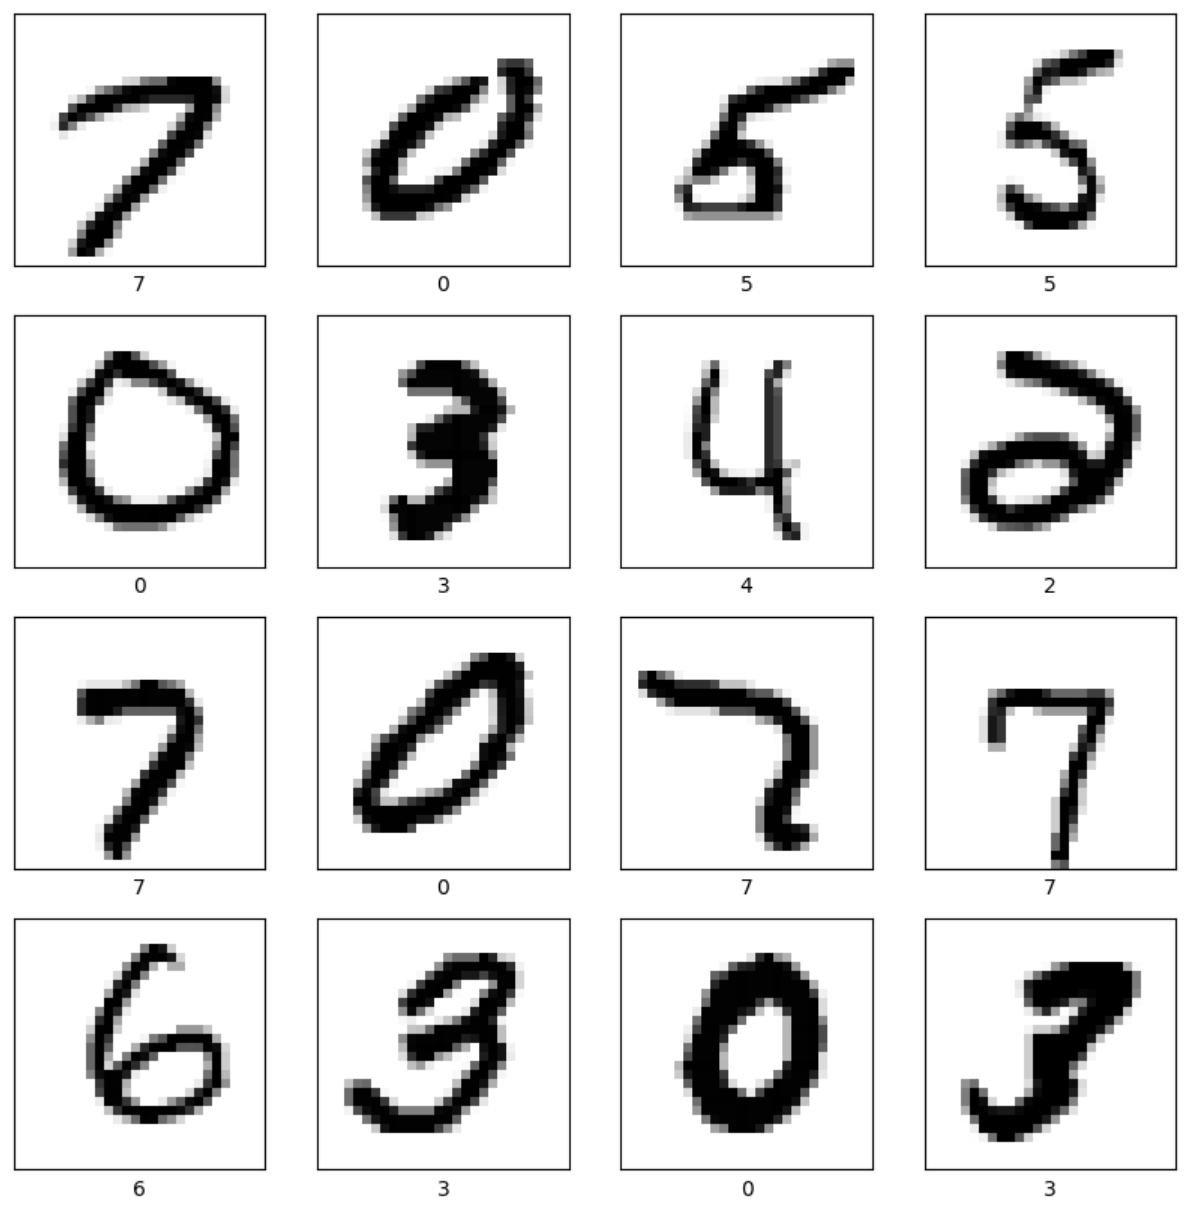
\includegraphics[width=0.8\linewidth]{images/data_visualization.png}
    \caption{16 images from the training data}
\end{figure}
